\chapter{Improving processor performance}
The performance of a processor is defined by the the time it takes to execute a program. This time span, called \emph{CPU time}, can be expressed as:

\begin{equation*}
  \text{CPU time} = \frac{\text{Seconds}}{\text{Program}} = \frac{\text{Clock cycles}}{\text{Program}} \cdot T_{ck}
\end{equation*}
where $T_{ck}$ is the clock period.

The first term can be decomposed further by computing the total number of instructions inside a program, called \emph{instruction count} (IC), which is known given the assembly code of the program. From this figure and the total number of clock cycles, the average number of \emph{clock cycles per instruction} (CPI)\footnote{Sometimes, also the inverse figure can be used, that is \emph{instructions per clock} (IPC).} can be derived. By factoring in these quantities, the final expression of CPU time is as follows \cite[p.~53]{hennessy17}:

\begin{equation}\label{eq:perf}
  \text{CPU time} = \text{IC} \cdot \text{CPI} \cdot T_{ck} 
\end{equation}

Equation \eqref{eq:perf} shows that the processor performance is directly and equally dependent on three factors:
\begin{itemize}
  \item Clock period, which depends mainly on the implementation technology and the microarchitectural choices (e.g. pipeline depth).
  \item Instruction count, which is determined for the most part by the ISA (see section \ref{sec:isas}) and compiler technology.
  \item CPI, which is dependant on both the ISA and the architecture.
\end{itemize}
The goal is then to minimize each of these terms, but it is evident that none of these parameters can be modified without affecting the others, as many design choices influence many of them.

\section{Instruction-level parallelism}
Earliest processors executed instructions one at a time, fetching a new one only after the previous has finished, leading to a number of clock cycles per instruction greater than one, and in particular equal to the number of stages an instruction must get through. These processors, where $\text{CPI} > 1$, are called \emph{subscalar}. To illustrate the situation, in the example of the classic 5-stage RISC pipeline (fetch, decode, execute, memory access, write back), a subscalar processor would execute three consecutive instructions as shown in figure \ref{fig:subscalar}, taking a total of 15 clock cycles.

\begin{figure}[hbtp]
  \centering
  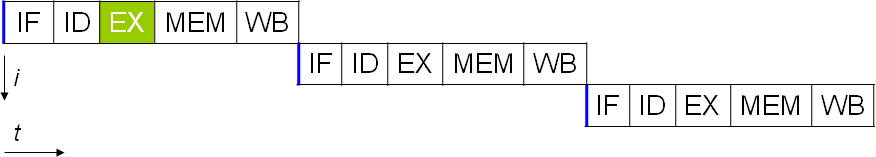
\includegraphics[width=0.8\textwidth]{img/subscalar.png}
  \caption{Subscalar processor}
  \label{fig:subscalar}
\end{figure}

Starting from the mid 80s, processor architects introduced \emph{pipelining} to improve performance by overlapping the execution of different instructions. This overlap means that at any given point in time there can be multiple instructions running in different stages of the processor, that is \emph{in parallel}, hence the term \emph{instruction-level parallelism} (ILP), which is a fundamental concept in developing techniques to enhance processor performance. For the same example of figure \ref{fig:subscalar}, a pipelined processor could theoretically achieve a CPI of 1, executing one instruction for each clock cycle (see figure \ref{fig:scalar}). Processors of this kind are called \emph{scalar}.

\begin{figure}[hbtp]
  \centering
  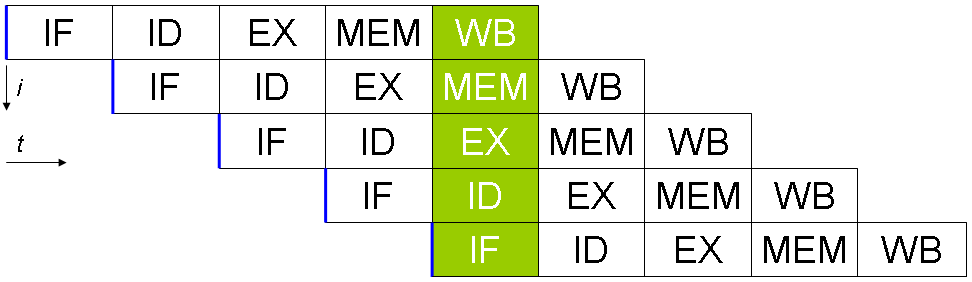
\includegraphics[width=0.8\textwidth]{img/scalar.png}
  \caption{Scalar processor}
  \label{fig:scalar}
\end{figure}

In practice however, data and control dependencies between successive instructions could cause hazards and force the pipeline to stall, causing CPI to rise once again at values greater than one. There are mainly three types of hazards that can take place in a pipelined processor:
\begin{itemize}
  \item \textbf{Structural hazards} arise when a hardware block is needed by two or more instructions at the same point in time. For instance, if a processor features only one memory block for both instructions and data, then two different instructions executing in the fetch and memory access stages could generate a structural hazard when trying to read from memory. Such hazards can either be easily solved (e.g. separate instruction and data memory in this example) or are known and accepted by the designers, given the limited hardware available.
  \item \textbf{Data hazards} in a simple pipelined processor occur when there is a \emph{data dependence} between instructions, that is one instruction needs to read a value that provided by a previous instruction. For example, in
      \begin{verbatim}
        add    x1, x2, x3
        sub    x4, x5, x1
      \end{verbatim}
      the \texttt{sub} instruction needs the value of register \texttt{x1} in the decode stage, but the previous \texttt{add} has not yet reached the write back stage and a data hazard is generated.
  \item \textbf{Control hazards} arise in the case of conditional flow changing instructions, such as branches, that prevent following instructions to be fetched until the new direction is resolved.
\end{itemize}

The real CPI a pipelined processor can achieve is then given by the sum of the ideal CPI and all the delays introduced by pipeline stalls caused by hazards io vole\cite[p.~168]{hennessy17}:
\begin{equation}\label{eq:pipe_cpi}
  \begin{split}
    \text{CPI}  & = \text{Ideal CPI} + \text{Structural stalls} + \text{Data hazard stalls} + \text{Control stalls} \\
                & = 1 + \text{Structural stalls} + \text{Data hazard stalls} + \text{Control stalls} > 1
  \end{split}
\end{equation}

Those hazards become more frequent and more expensive to manage the more pipeline stages are introduced and that is a clear example of a tradeoff between two factors of the performance equation \eqref{eq:perf}: a deeper pipeline shortens the critical path and thus reduces the clock period, but at the same time it increases the CPI. That is the reason why designers at some point had to find other architectural solutions to improve performance.

\subsection{Multiple-issue processors}
A processor featuring a single execution pipeline can only achieve a theoretical CPI of 1, but by duplicating the pipeline to include multiple execution units more than one instruction per clock cycle could be delivered. That is the idea that lies behind \emph{multiple-issue} processors, that exploit ILP by executing independent instructions on separate execution pipelines.

Instructions that can be issued independently to the different pipelines are selected among a so called \emph{basic block}, that is a sequence of instructions comprised between single entry and exit points (i.e. with no branches or jumps in between). Recalling the examples of the previous section, figure \ref{fig:superscalar} shows the execution scheme for a multiple issue processor.

\begin{figure}[hbtp]
  \centering
  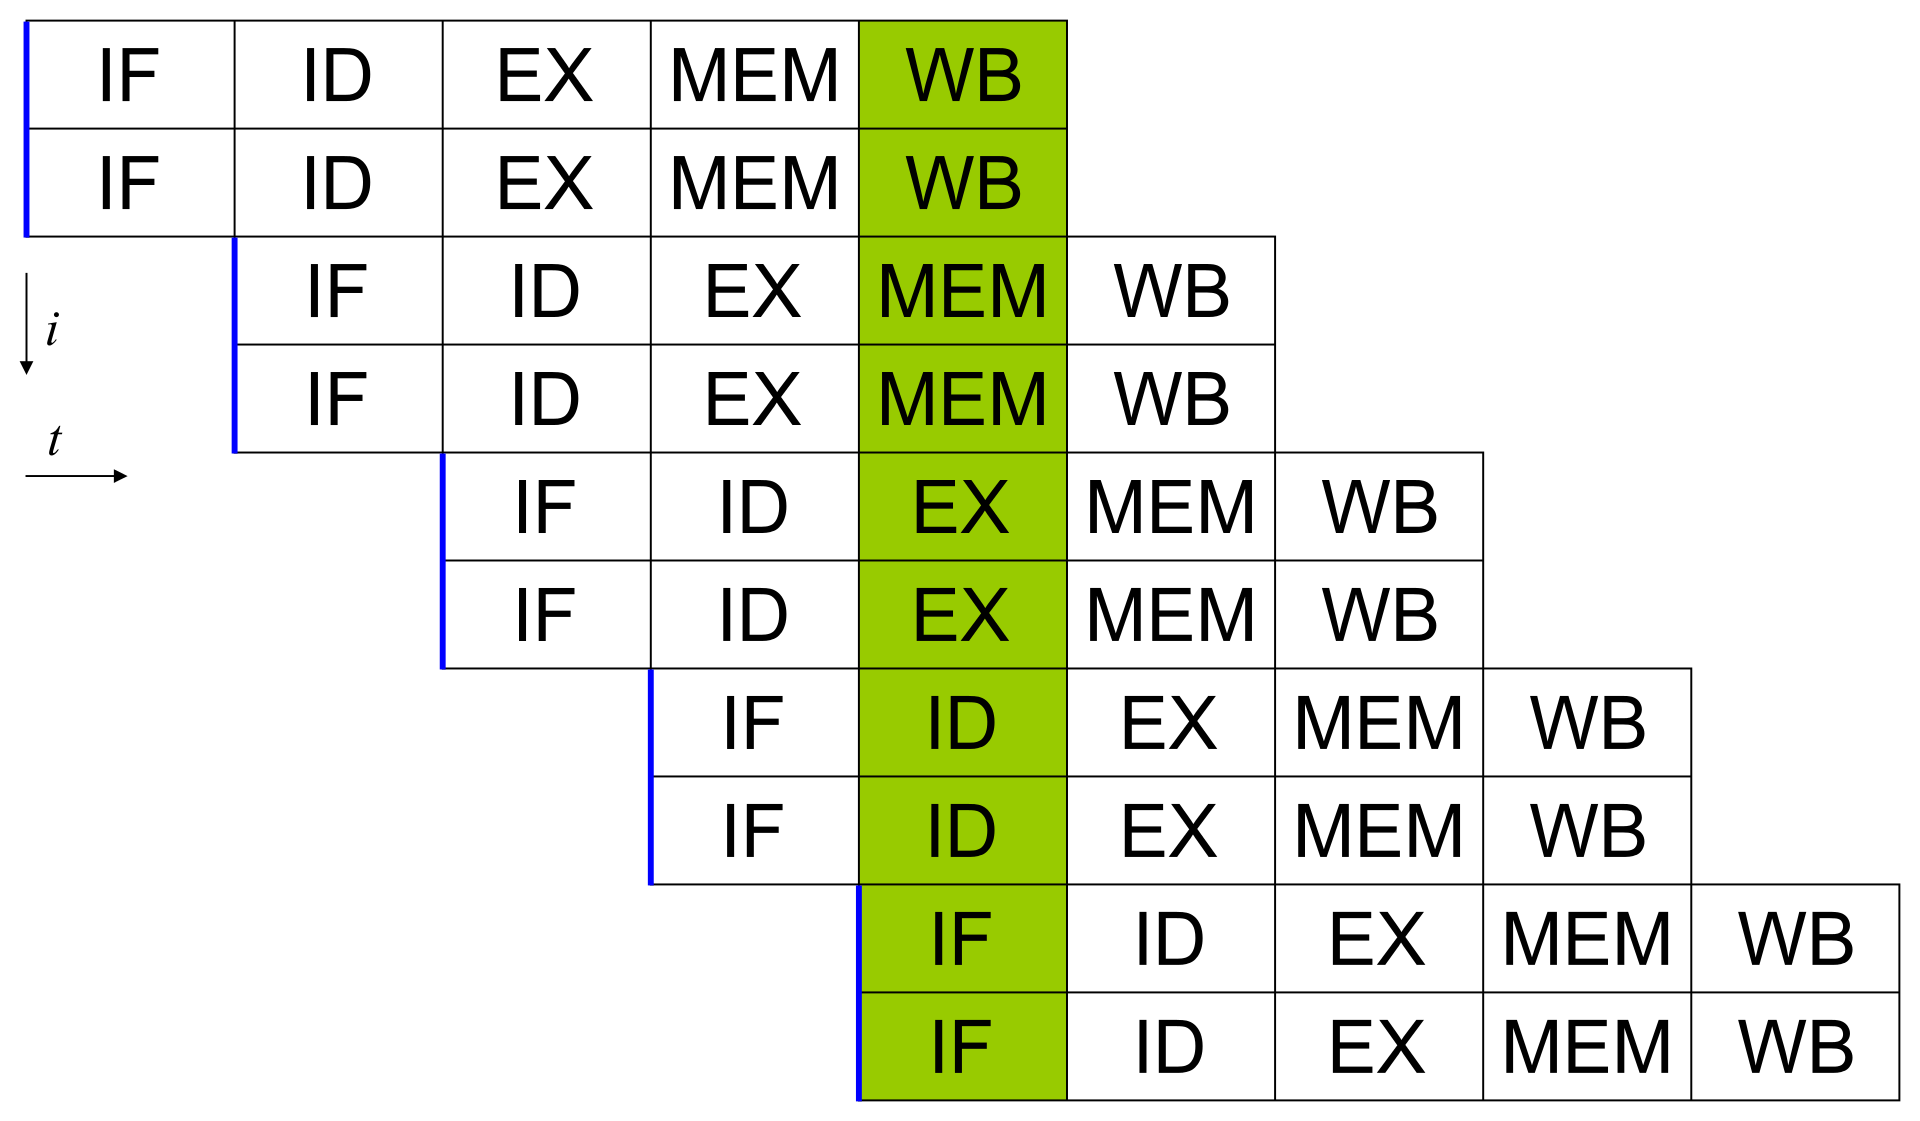
\includegraphics[width=0.8\textwidth]{img/superscalar.png}
  \caption{Multiple-issue processor with two pipelines}
  \label{fig:superscalar}
\end{figure}

Two main different approaches exist to multiple issue processors:
\begin{itemize}
  \item \textbf{VLIW (Very Long Instruction Word)} processors, also known as \emph{static} multiple-issue, rely on software to discover ILP chances at compile time, thus avoiding increased hardware complexity. The compiler groups instructions that can be executed in parallel in a single long packet-like instruction (hence the name VLIW), that is then split and issued to the different execution units at run time. Despite many efforts, however, such static techniques reveal efficient only for specific applications presenting a high level of data parallelism \cite[p.~168]{hennessy17}, mainly because the compiler software needs a perfect knowledge of the underlying architecture in order to efficiently exploit ILP.
  \item \textbf{Superscalar} processors, also known as \emph{dynamic} multiple-issue, on the other hand, rely on dedicated hardware to exploit ILP at run time. Instructions belonging to a basic block are inserted into a \emph{window of execution} (WOE), from where instruction that can run in parallel thanks to no data dependence are selected and issued to the respective following pipeline stages. This dynamic approach has been shown to work better than a static one, at the cost of a significant hardware complexity overhead.
\end{itemize}

Multiple-issue processors can achieve a CPI lower than 1 (usually expressed at this point as IPC, greater than 1) thanks to duplicate hardware units that also lower the impact of structural hazards, but they are nonetheless subject to data and control hazards. Instructions belonging to the same basic block are very likely to depend upon one another, as they are part of the same piece of program, and as such the amount of ILP in contiguous instructions of a basic block is usually very small, neglecting almost totally the performance improvements of multiple issues.

\section{Dynamic scheduling}

\section{Speculation}

